\documentclass[a4paper,12pt]{article}
\usepackage[T2A]{fontenc}
\usepackage[utf8]{inputenc}
\usepackage[top=2cm, bottom=2cm, right=2cm, left=2cm]{geometry}
\usepackage[russian]{babel}
\usepackage{pscyr}
\usepackage{indentfirst}
\usepackage{graphicx}
\usepackage{epstopdf}
\usepackage{amstext}
\usepackage{amssymb}
\usepackage{amsmath}
\usepackage{cmap}
\usepackage{enumitem}
\usepackage{multirow}
\pdfminorversion=6
%\input{environment}
%\linespread{1.3}
\tolerance=1000 
\hfuzz=0pt
\parindent=1.27cm
\usepackage{subcaption}
\captionsetup[table]{name = Таблица, labelsep = endash, justification=raggedright, singlelinecheck=false}
\captionsetup[figure]{name = Рисунок, labelsep = endash}
%\sloppy
\RequirePackage{caption}
\DeclareCaptionLabelSeparator{defffis}{ -- }
\captionsetup{justification=centering,labelsep=defffis}

\graphicspath{{images/}}

\begin{document}
	\newcommand\tline[2]{$\underset{\text{#1}}{\text{\underline{\hspace{#2}}}}$}
	\begin{titlepage}
		\centering
		{\fontsize{12pt}{5cm}\selectfont \bfseries Министерство образования и науки Российской Федерации} \\ \vspace{0.5cm}
		{\fontsize{7pt}{5cm}\selectfont ФЕДЕРАЛЬНОЕ ГОСУДАРСТВЕННОЕ АВТОНОМНОЕ ОБРАЗОВАТЕЛЬНОЕ УЧРЕЖДЕНИЕ ВЫСШЕГО ПРОФЕССИОНАЛЬНОГО ОБРАЗОВАНИЯ} \\ 
		\vspace{1cm}
		{\fontsize{12pt}{5cm}\selectfont \bfseries САНКТ-ПЕТЕРБУРГСКИЙ УНИВЕРСИТЕТ ИНФОРМАЦИОННЫХ ТЕХНОЛОГИЙ, МЕХАНИКИ И ОПТИКИ} \\ \vspace{1.5cm}

		{\fontsize{14pt}{5cm}\selectfont Кафедра \hspace{1cm} \underline{Систем Управления и Информатики}  \hspace{1cm} Группа \underline{Р3340}} \\ 
		\vspace{2cm}

		{\fontsize{20pt}{5cm}\selectfont \bfseries Лабораторная работа №10} \\
		{\fontsize{20pt}{5cm}\selectfont \bfseries “Исследование математической модели электромеханического объекта управления”} \\
		{\fontsize{14pt}{5cm}\selectfont Вариант - 5} \\
		\vspace{1.5cm}

		\flushleft

		{Выполнил \hspace{2cm} \tline{(фамилия, и.о.)}{9cm} (подпись)} \\
		\vspace{2cm}

		{Проверил \hspace{2cm} \tline{(фамилия, и.о.)}{9cm} (подпись)} \\
		\vspace{5cm}

		"\underline{\hspace{0.7cm}}"\hspace{0.2cm}\underline{\hspace{2cm}}\hspace{0.2cm}20\underline{\hspace{0.7cm}}г. \hspace{2cm} Санкт-Петербург, \hspace{2cm} 20\underline{\hspace{0.7cm}}г. \\ \vspace{1cm}

		Работа выполнена с оценкой \hspace{1cm} \underline{\hspace{8cm}} \\ 
		\vspace{1cm}
		Дата защиты "\underline{\hspace{0.7cm}}"\hspace{0.2cm}\underline{\hspace{2cm}}\hspace{0.2cm}20\underline{\hspace{0.7cm}}г.

	\end{titlepage}
	\paragraph{Цель работы.}  Изучение математических моделей и исследование характеристик электромеханического объекта управления, построенного на основе электродвигателя постоянного тока независимого возбуждения.
	\paragraph {Исходные данные:} Представлены в таблице \ref{t_1}
	\begin{table}[h]
		\caption{Исходные данные}
		\renewcommand{\arraystretch}{2} 
		\renewcommand{\tabcolsep}{0.35cm}
		\begin{center}
			\begin{tabular}{|c|c|c|c|c|c|c|c|c|c|}
				\hline
				$U_H$, В & $n_0$, об/мин & $I_H$, А & $M_H$, Нм & $R$, Ом & $T_{\text{я}}$, мс &$J_{\text{д}}$, кг$\cdot\text{м}^2$ & $T_y$, мс & $i_p$ & $J_{\text{м}}$, кг$\cdot\text{м}^2$ \\ \hline
				120 & 6000 & 21 & 4 & 0.53 & 8 & 1.9$\cdot10^{-3}$ & 8 & 40 & 5.75 \\ \hline
			\end{tabular}
		\end{center}
		\label{t_1}
	\end{table}
	
	\paragraph {} Рассчет необходимых параметров модели:\\
	
	\noindent
	\begin{gather}
	J_{\text{р}}=0.2\cdot J_{\text{д}}=3.8\cdot10^{-4}\\
	w_0=n_0\cdot\displaystyle \frac{2\pi}{60}=628\\
	k_e=\frac{U_H}{w_0}=0.191\\
	k_{\text{м}}=\frac{M_H}{I_H}=0.1905\\
	J_{\small\sum}\normalsize =J_{\text{д}}+J_{\text{р}}+\frac{J_{\text{м}}}{{i_p}^2}=0.0059\\
	K_y=\frac{U_H}{U_m}=12\\
	K=\frac{K_y}{k_e\cdot i_p}=1.57\\
	K_f=\frac{R}{k_m\cdot k_e\cdot {i_p}^2}=0.0091\\
	T_M=\frac{R\cdot J_{\sum}}{k_m\cdot k_e}=0.085
	\end{gather}
	
	\noindent Коэффициенты передачи измерительных устройств:\\
	
	
	\begin{gather}
	K_u=0.1667\\
	K_i=0.1119\\
	K_w=0.0318\\
	K_\alpha=1.4047
	\end{gather}
	\newpage
	\begin{center}			
	\section{Исследование полной математической модели ЭМО}
	\end{center}
		\paragraph {} Схема моделирования представлена на рисунке \ref{s_1}
		
		\begin{figure}[h]
			\renewcommand{\figurename}{Рисунок}
			\centering
			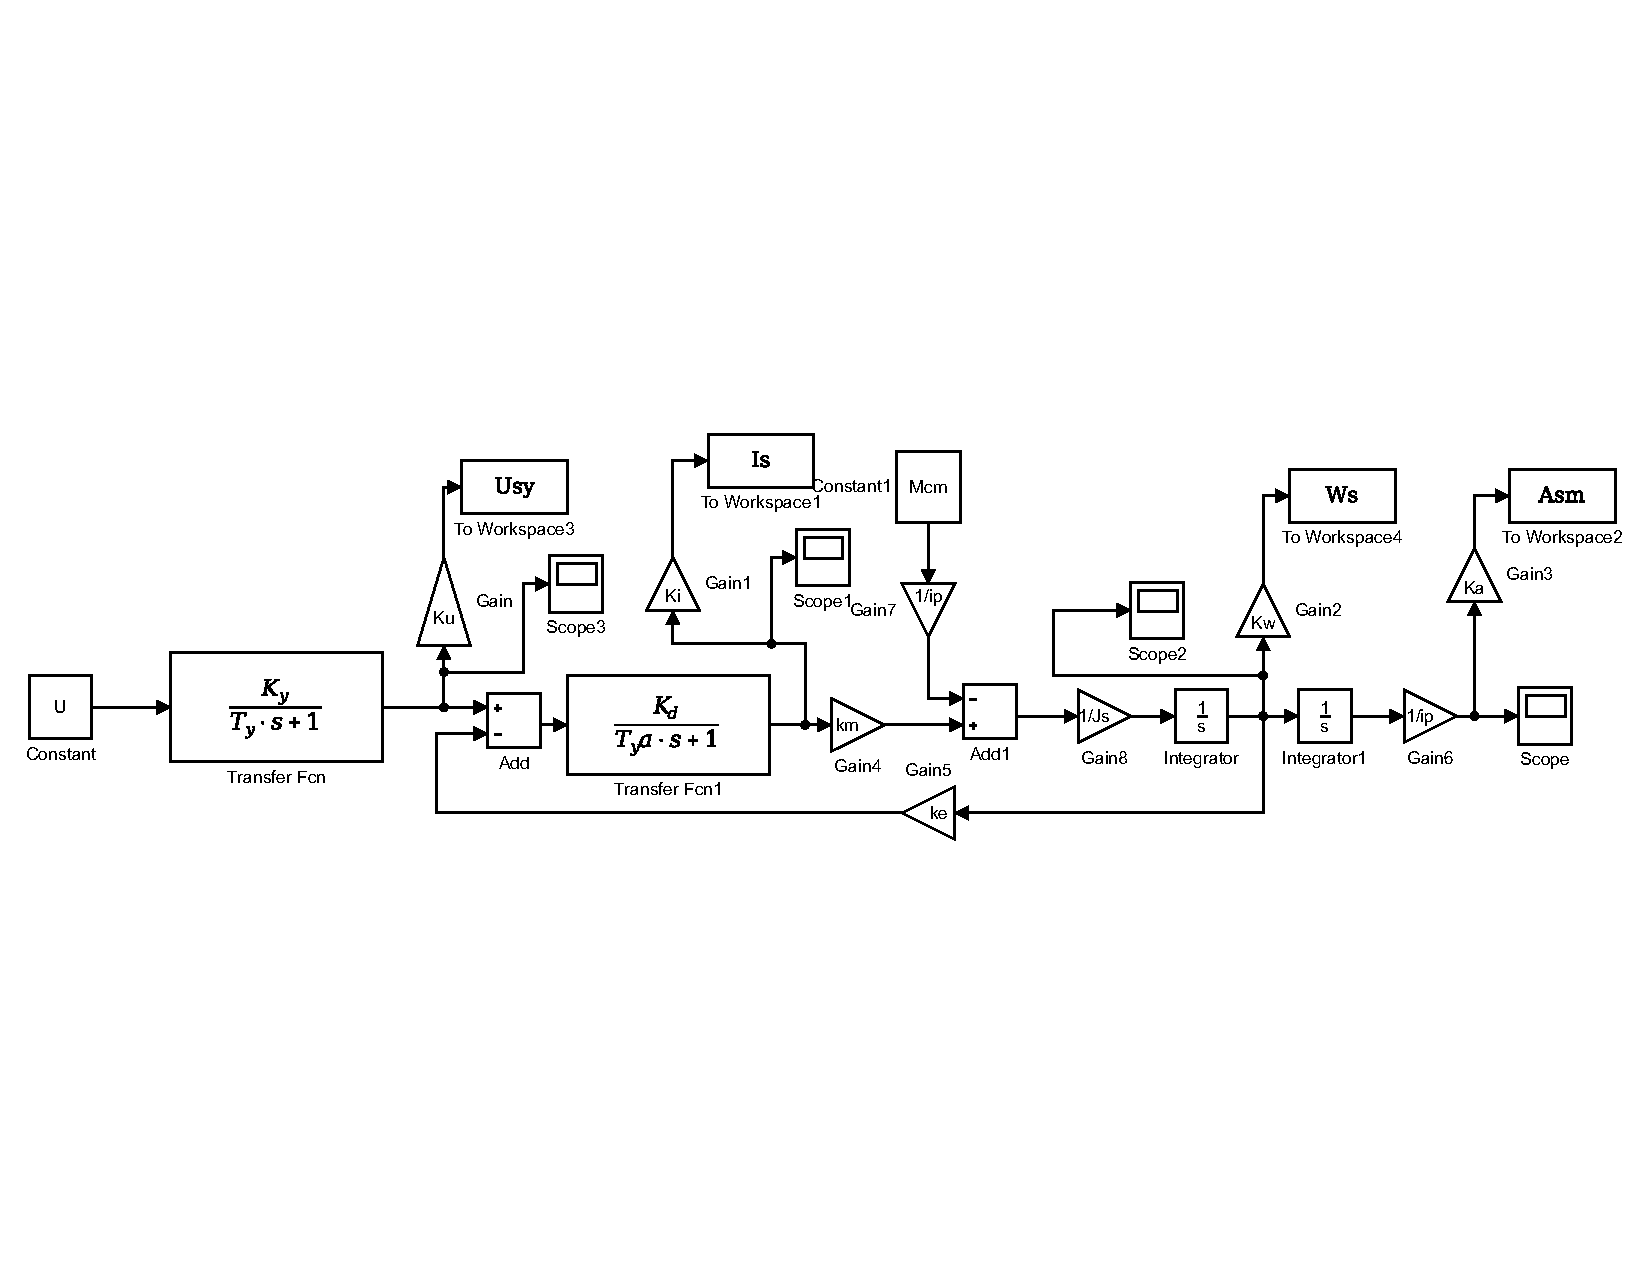
\includegraphics[width=6in]{Lab10full.pdf}
			\caption{Схема моделирования}
			\label{s_1}
		\end{figure}
	%\newpage
	\paragraph {} Графики переходных процессов при $U=5$ и $M_{\text{см}}=0$ представлены на рисунке \ref{s_2}
	
		\begin{figure}[h!]
			\renewcommand{\figurename}{Рисунок}
			\centering
			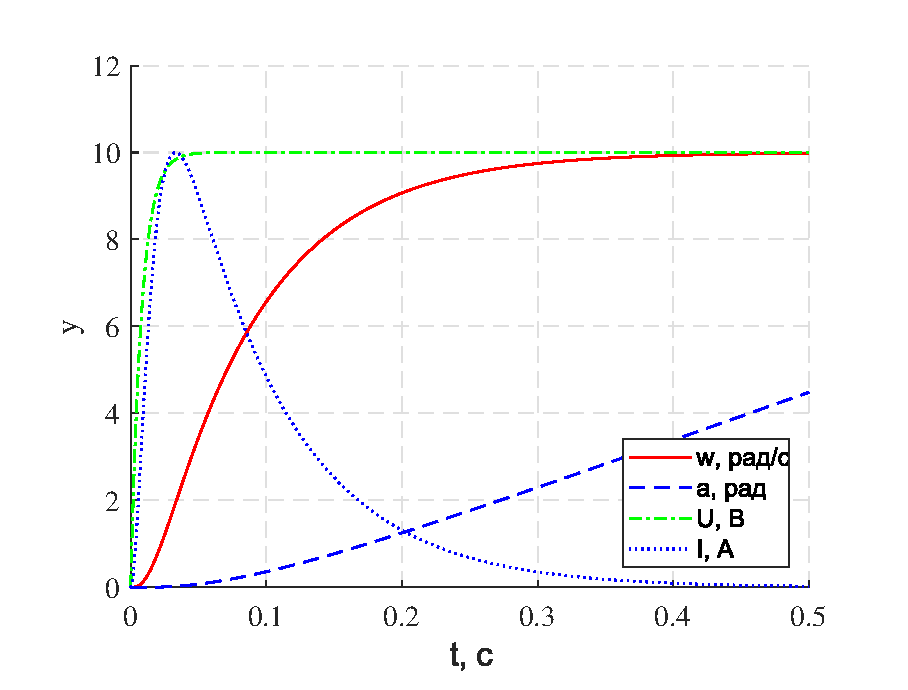
\includegraphics[width=4in]{ph1.eps}
			\caption{Переходные процессы}
			\label{s_2}
		\end{figure}
	\newpage
	\subsection{Исследование влияния момента сопротивления $M_{\text{см}}$ на вид переходных процессов}~~\\
		\paragraph {} Графики переходных процессов при различных $M_{\text{см}}$ для каждого из исследуемых значений представлены на рисунке \ref{s_3}\\
		
		\begin{figure}[h!]
			\renewcommand{\figurename}{Рисунок}
			\begin{minipage}[h]{0.47\linewidth}
				\center{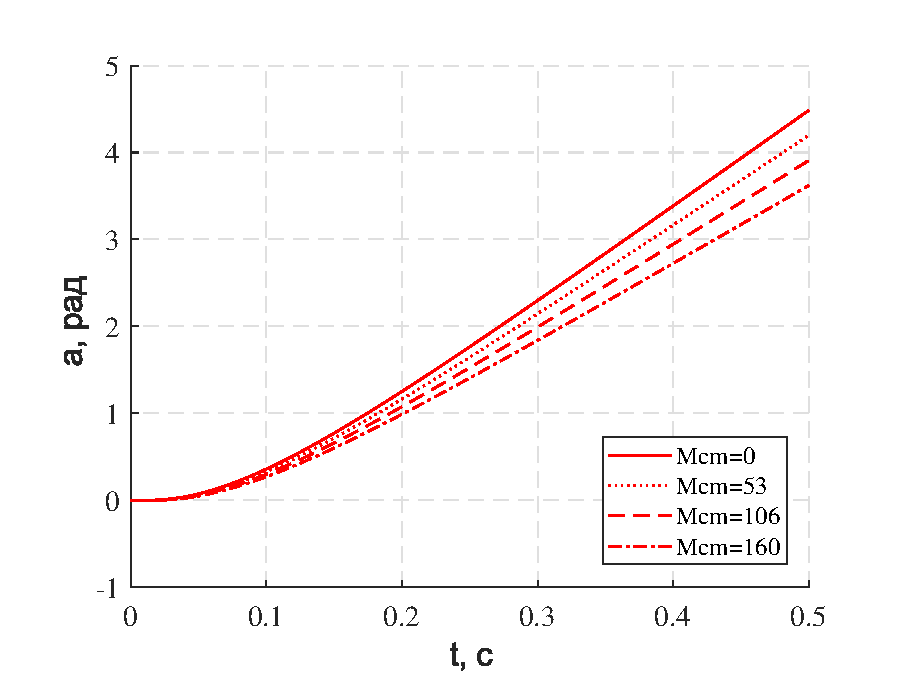
\includegraphics[width=1\linewidth]{a_pri_mcm.eps}} a) \\
			\end{minipage}
			\hfill
			\begin{minipage}[h]{0.47\linewidth}
				\center{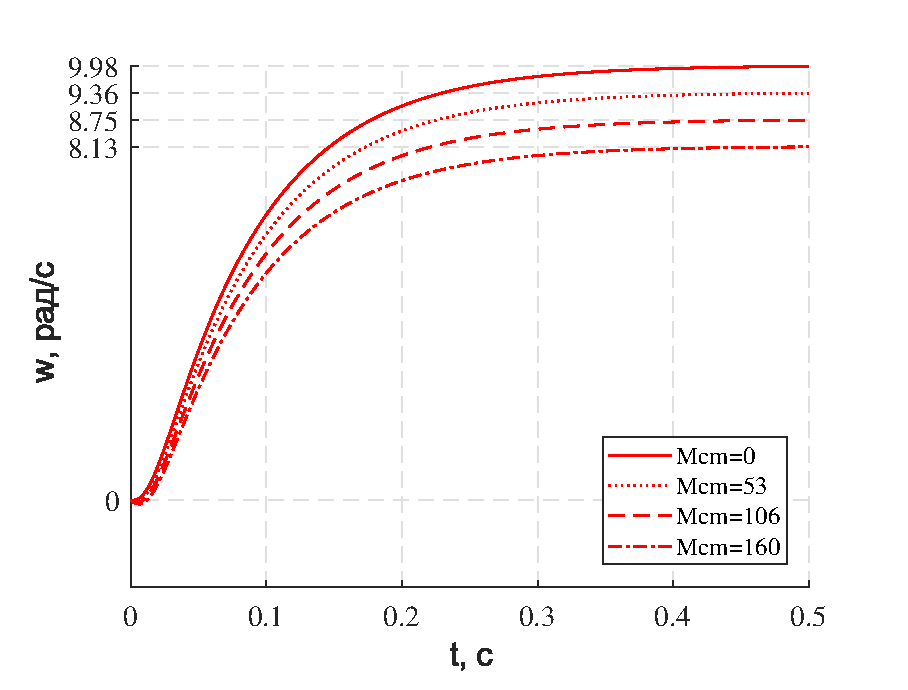
\includegraphics[width=1\linewidth]{w_pri_mcm.eps}} \\b)
			\end{minipage}
			\vfill
			\begin{minipage}[h]{0.47\linewidth}
				\center{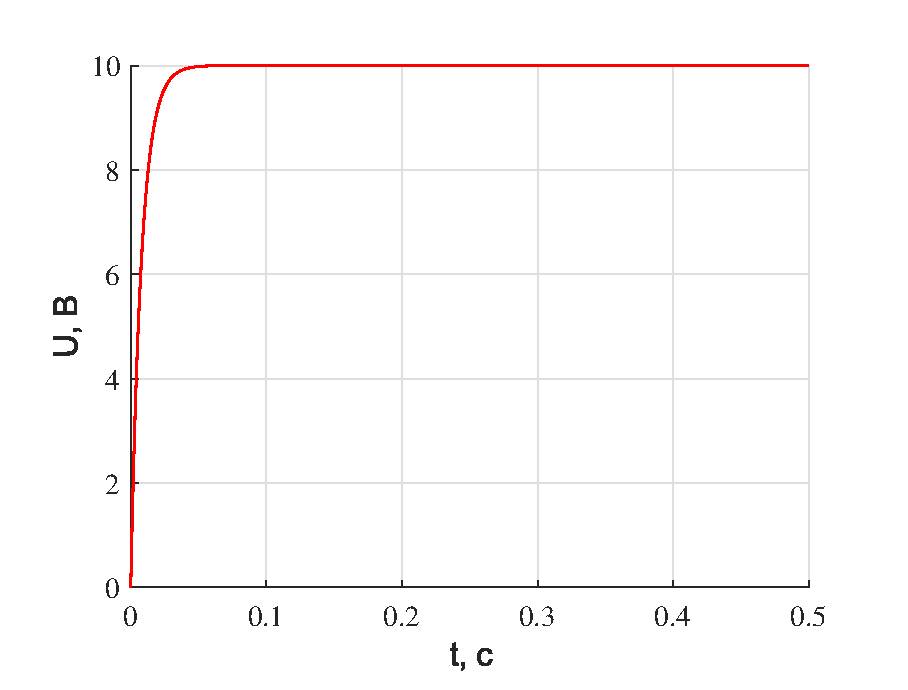
\includegraphics[width=1\linewidth]{u_pri_mcm.eps}} c) \\
			\end{minipage}
			\hfill
			\begin{minipage}[h]{0.47\linewidth}
				\center{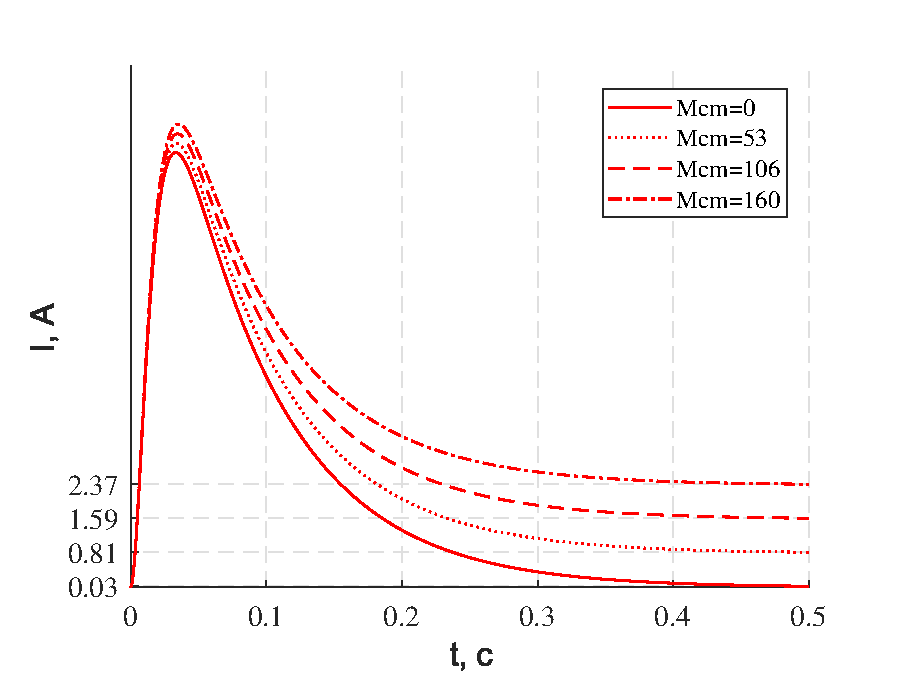
\includegraphics[width=1\linewidth]{i_pri_mcm.eps}} d) \\
			\end{minipage}
			\caption{Переходные процессы: a) угол поворота, b)
				скорость вращения, c) напряжение, d) сила тока}
			\label{s_3}
		\end{figure}
	\newpage
	\paragraph{}Рассчитаем значения времени переходного процесса $t_\text{п}$ и установившееся значение при различных $M_{\text{см}}$ для $w$ и $I$. Результаты представлены в таблице \ref{t_2}
	 \begin{table}[h]
		\caption{Данные моделирования}
		\renewcommand{\arraystretch}{2} 
		\renewcommand{\tabcolsep}{0.5cm}
		\begin{center}
			\begin{tabular}{|c|c|c|c|c|}
				\hline
				\multirow{2}*{$M_{\text{см}}$} & \multicolumn{2}{|c|}{$t_\text{п}$} & \multicolumn{2}{|c|}{Установившееся значение} \\ \cline{2-5}
				& $w$ & $I$ & $w$ & $I$ \\ \hline
				0 & 0.25 & 0.5 & 9.98 & 0.03\\ \hline
				53 & 0.25 & 0.43 & 9.36 & 0.8\\ \hline
				106 & 0.25 & 0.39 & 8.75 & 1.6\\ \hline
				160 & 0.25 & 0.36 & 8.13 & 2.37\\ \hline
				
			\end{tabular}
		\end{center}
		\label{t_2}
	\end{table}
	\newpage
	\subsection{Исследование влияния момента инерции механизма $J_{\text{м}}$ на вид переходных процессов}~~\\
	\paragraph {} Графики переходных процессов при различных $J_{\text{м}}$ для каждого из исследуемых значений представлены на рисунке \ref{s_4}\\
	
	\begin{figure}[h!]
		\renewcommand{\figurename}{Рисунок}
		\begin{minipage}[h]{0.47\linewidth}
			\center{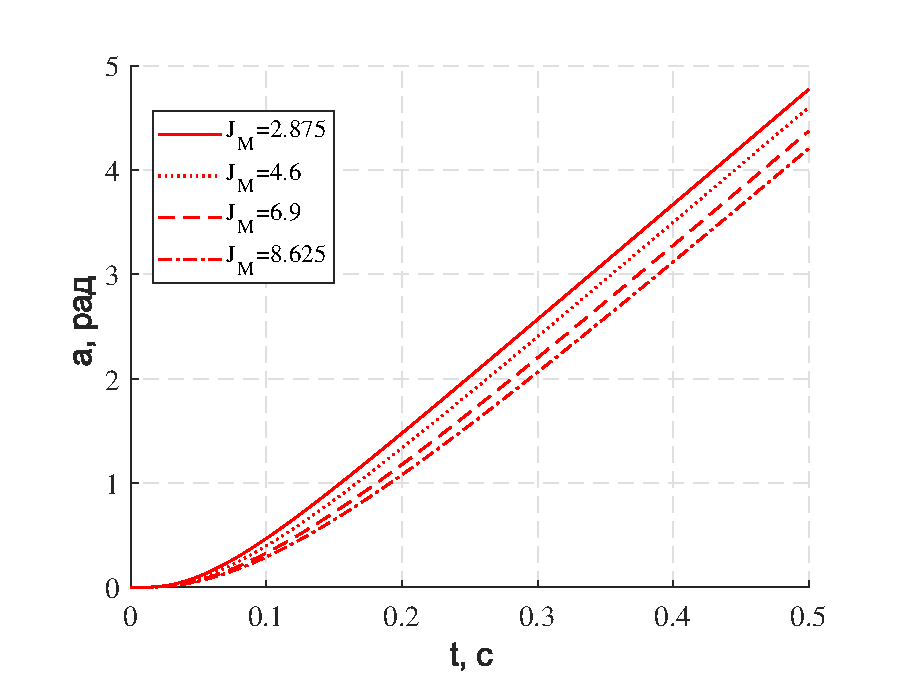
\includegraphics[width=1\linewidth]{a_pri_jm.eps}} a) \\
		\end{minipage}
		\hfill
		\begin{minipage}[h]{0.47\linewidth}
			\center{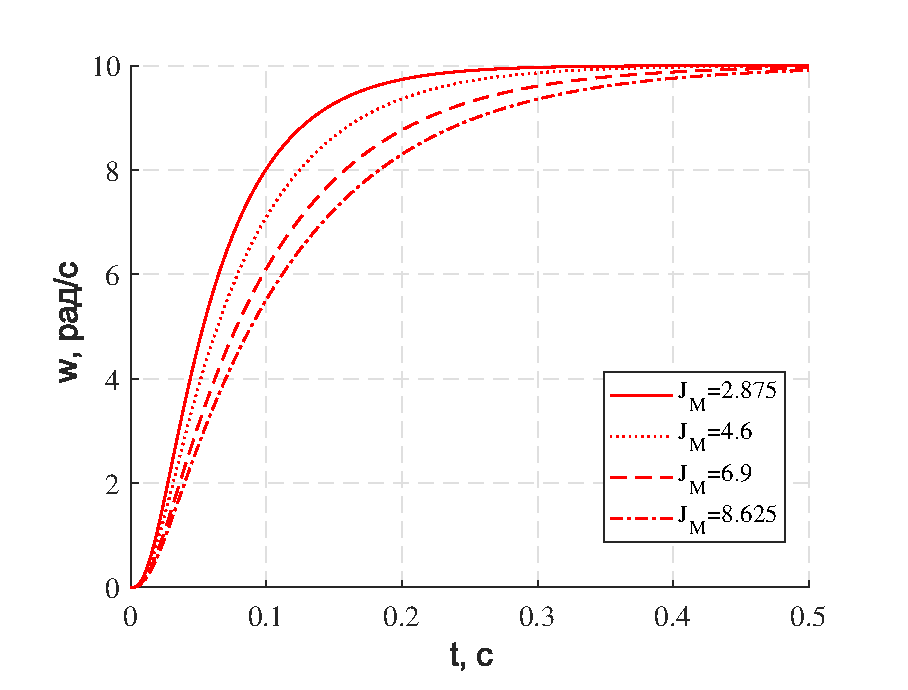
\includegraphics[width=1\linewidth]{w_pri_jm.eps}} \\b)
		\end{minipage}
		\vfill
		\begin{minipage}[h]{0.47\linewidth}
			\center{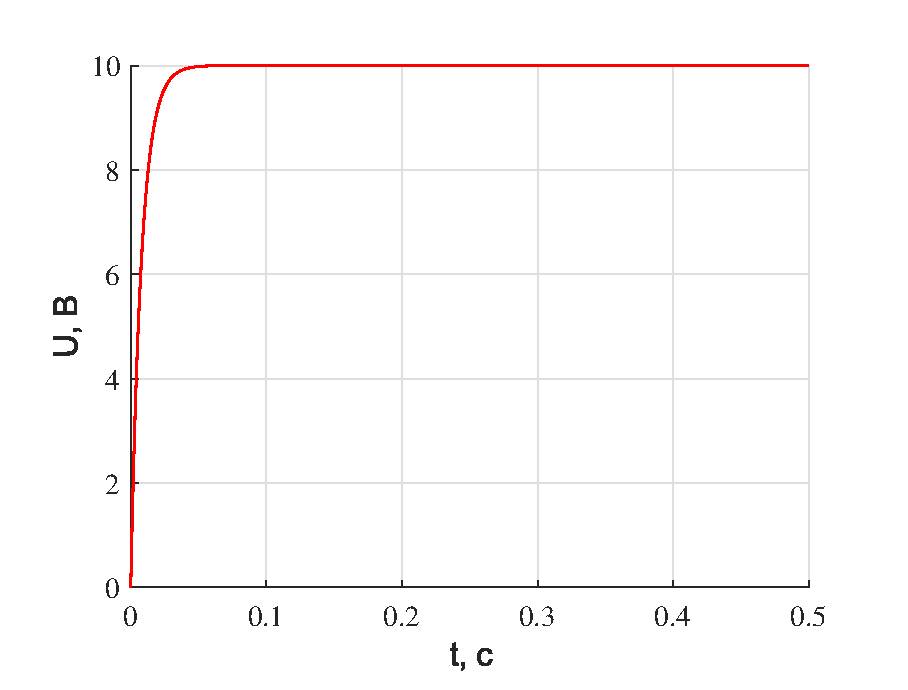
\includegraphics[width=1\linewidth]{u_pri_jm.eps}} c) \\
		\end{minipage}
		\hfill
		\begin{minipage}[h]{0.47\linewidth}
			\center{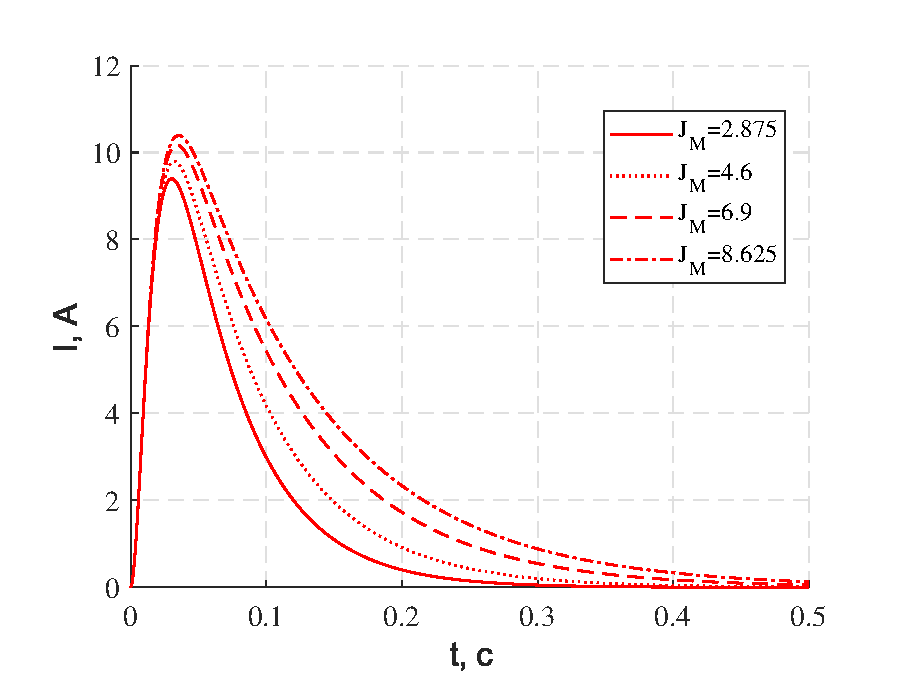
\includegraphics[width=1\linewidth]{i_pri_jm.eps}} d) \\
		\end{minipage}
		\caption{Переходные процессы: a) угол поворота, b)
			скорость вращения, c) напряжение, d) сила тока}
		\label{s_4}
	\end{figure}
	\newpage
	\paragraph{}Рассчитаем значения времени переходного процесса $t_\text{п}$ и установившееся значение при различных $J_{\text{м}}$ для $w$ и $I$. Результаты представлены в таблице \ref{t_3}
	\begin{table}[h]
		\caption{Данные моделирования}
		\renewcommand{\arraystretch}{2} 
		\renewcommand{\tabcolsep}{0.5cm}
		\begin{center}
			\begin{tabular}{|c|c|c|c|c|}
				\hline
				\multirow{2}*{$J_{\text{м}}$} & \multicolumn{2}{|c|}{$t_\text{п}$} & \multicolumn{2}{|c|}{Установившееся значение} \\ \cline{2-5}
				& $w$ & $I$ & $w$ & $I$ \\ \hline
				2.875 & 0.17 & 0.49 & 9.99 & 0\\ \hline
				4.6 & 0.22 & 0.49 & 9.99 & 0\\ \hline
				6.9 & 0.27 & 0.49 & 9.96 & 0.06\\ \hline
				8.625 & 0.31 & 0.49 & 9.13 & 0.12\\ \hline
				
			\end{tabular}
		\end{center}
		\label{t_3}
	\end{table}
	
	\newpage
	
	\subsection{Исследование влияния передаточного числа $i_p$ на вид переходных процессов при $M_{\text{см}}=0$ и $M_{\text{см}}=80$}~~\\
	\paragraph {При $M_{\text{см}}=0$}~\\ 
	
	Графики переходных процессов при различных $i_p$ для каждого из исследуемых значений представлены на рисунке \ref{s_5}\\
	
	\begin{figure}[h!]
		\renewcommand{\figurename}{Рисунок}
		\begin{minipage}[h]{0.47\linewidth}
			\center{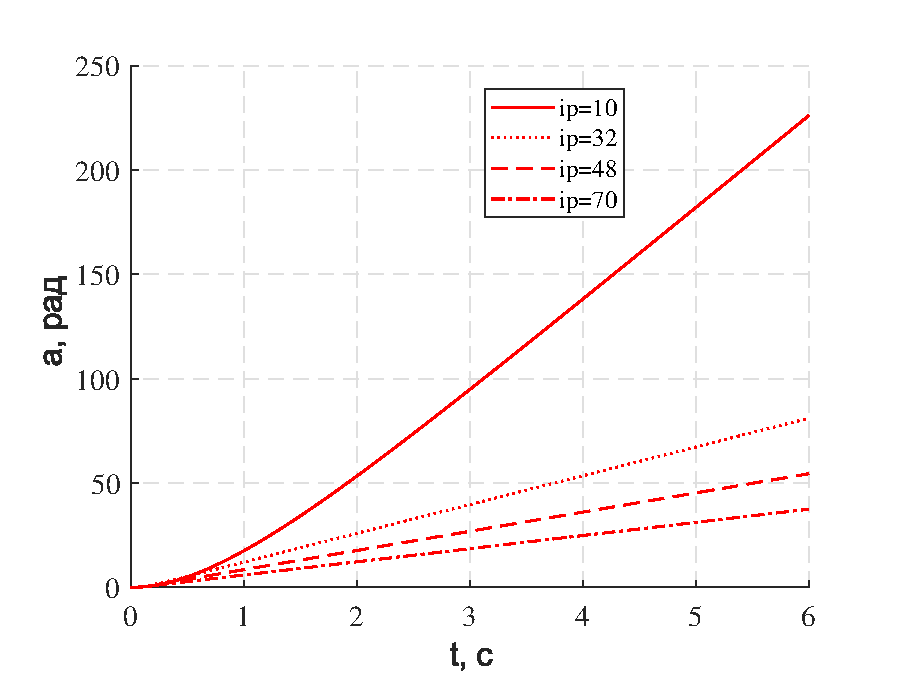
\includegraphics[width=1\linewidth]{new_a_ip_m0.eps}} a) \\
		\end{minipage}
		\hfill
		\begin{minipage}[h]{0.47\linewidth}
			\center{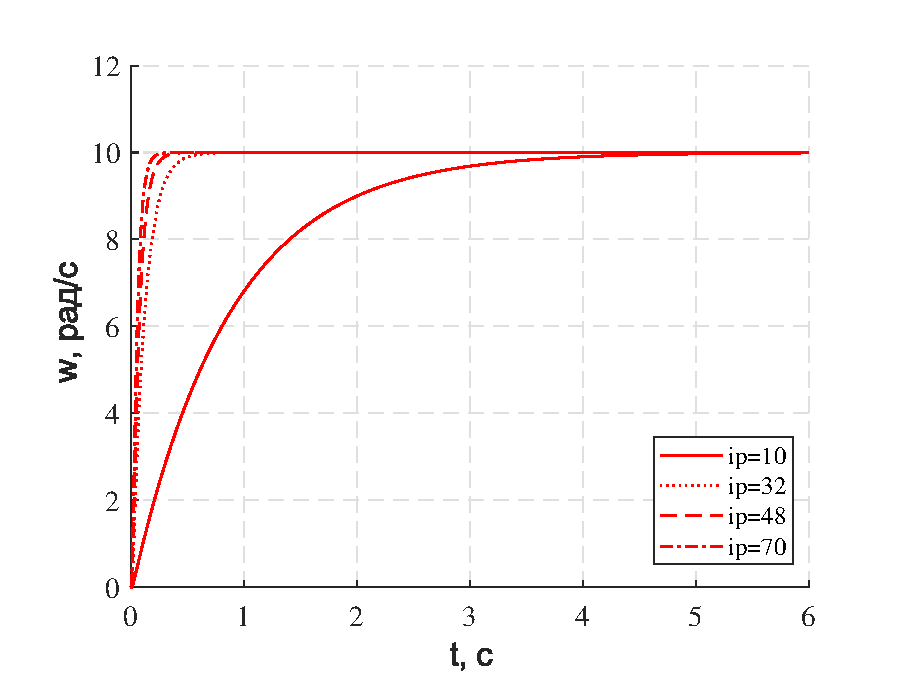
\includegraphics[width=1\linewidth]{new_w_ip_m0.eps}} \\b)
		\end{minipage}
		\vfill
		\begin{minipage}[h]{0.47\linewidth}
			\center{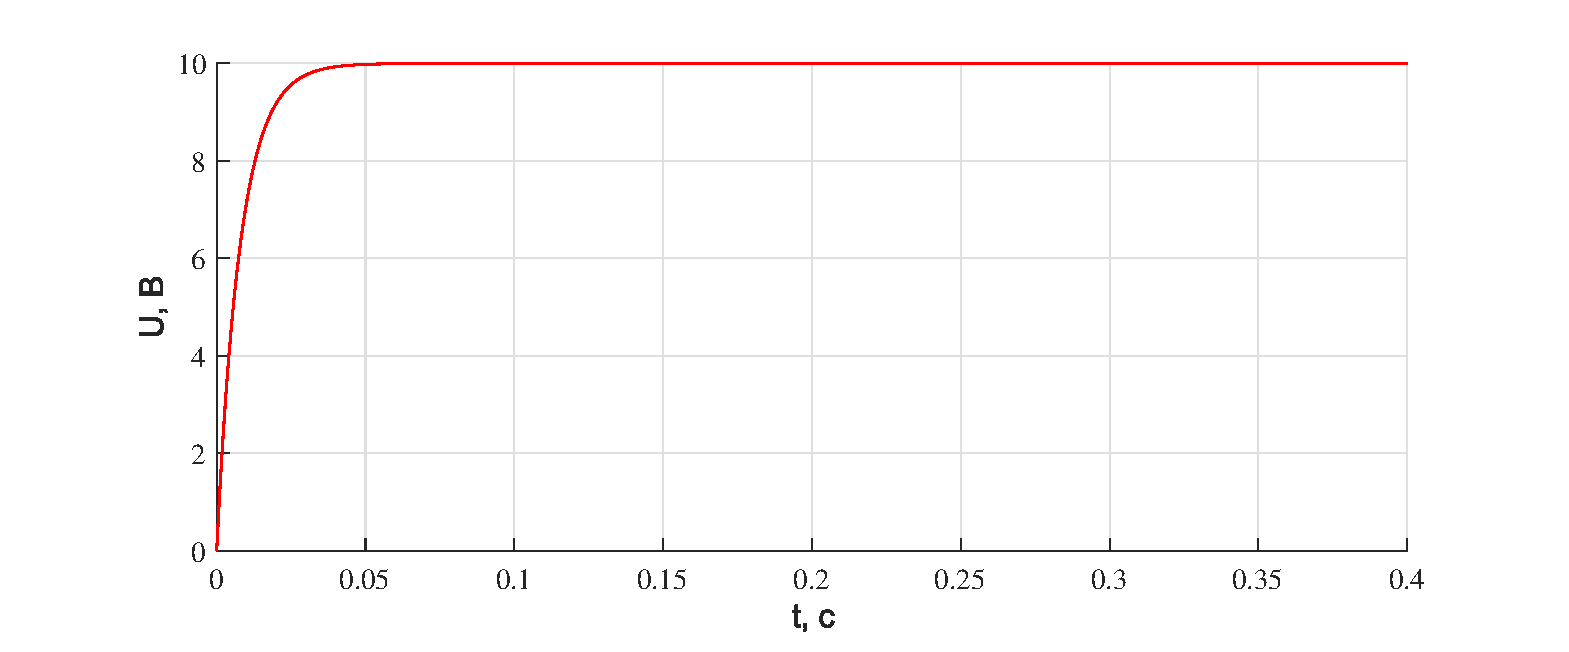
\includegraphics[width=1\linewidth]{new_u_ip_m0.eps}} c) \\
		\end{minipage}
		\hfill
		\begin{minipage}[h]{0.47\linewidth}
			\center{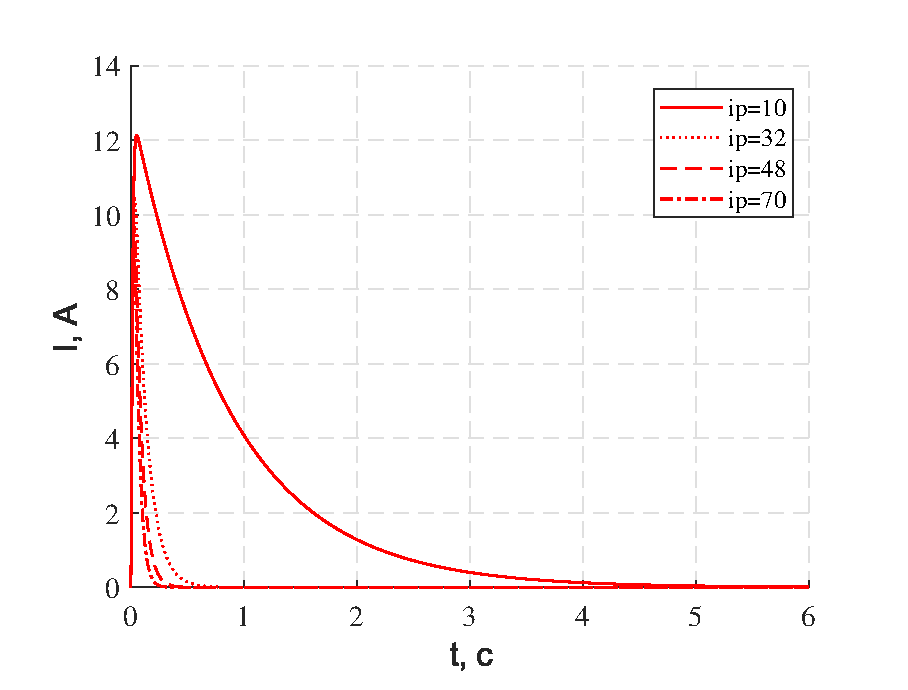
\includegraphics[width=1\linewidth]{new_i_ip_m0.eps}} d) \\
		\end{minipage}
		\caption{Переходные процессы: a) угол поворота, b)
			скорость вращения, c) напряжение, d) сила тока}
		\label{s_5}
	\end{figure}
	\newpage
	\paragraph{}Рассчитаем значения времени переходного процесса $t_\text{п}$ и установившееся значение при различных $i_p$ для $w$ и $I$. Результаты представлены в таблице \ref{t_4}
	\begin{table}[h]
		\caption{Данные моделирования}
		\renewcommand{\arraystretch}{2} 
		\renewcommand{\tabcolsep}{0.5cm}
		\begin{center}
			\begin{tabular}{|c|c|c|c|c|}
				\hline
				\multirow{2}*{$i_p$} & \multicolumn{2}{|c|}{$t_\text{п}$} & \multicolumn{2}{|c|}{Установившееся значение} \\ \cline{2-5}
				& $w$ & $I$ & $w$ & $I$ \\ \hline
				10 & 2.58 & 5.95 & 10 & 0\\ \hline
				32 & 0.34 & 3.45 & 10 & 0\\ \hline
				48 & 0.2 & 2 & 10 & 0\\ \hline
				70 & 0.14 & 1.37 & 10 & 0\\ \hline
				
			\end{tabular}
		\end{center}
		\label{t_4}
	\end{table}
	\newpage
	\paragraph {При $M_{\text{см}}=80$}~\\ 
	
	Графики переходных процессов при различных $i_p$ для каждого из исследуемых значений представлены на рисунке \ref{s_6}\\
	
	\begin{figure}[h!]
		\renewcommand{\figurename}{Рисунок}
		\begin{minipage}[h]{0.47\linewidth}
			\center{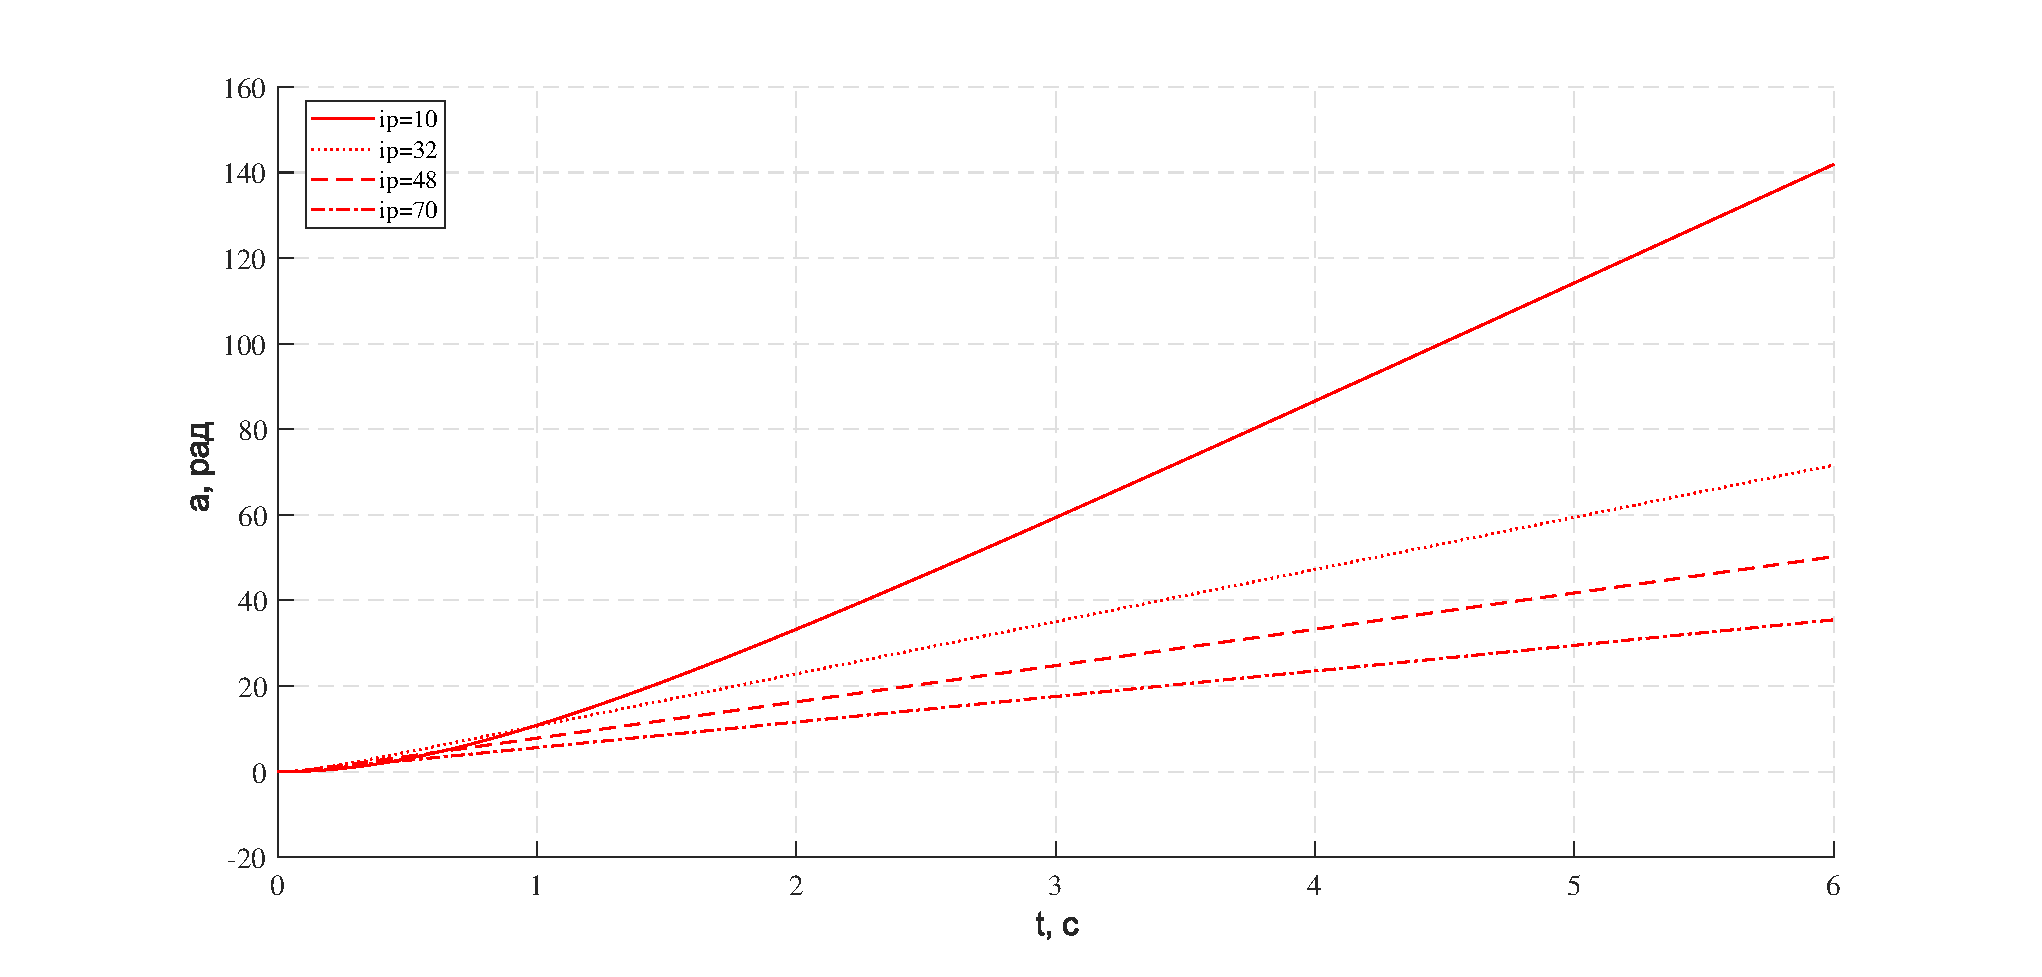
\includegraphics[width=1\linewidth]{new_a_ip_m80.eps}} a) \\
		\end{minipage}
		\hfill
		\begin{minipage}[h]{0.47\linewidth}
			\center{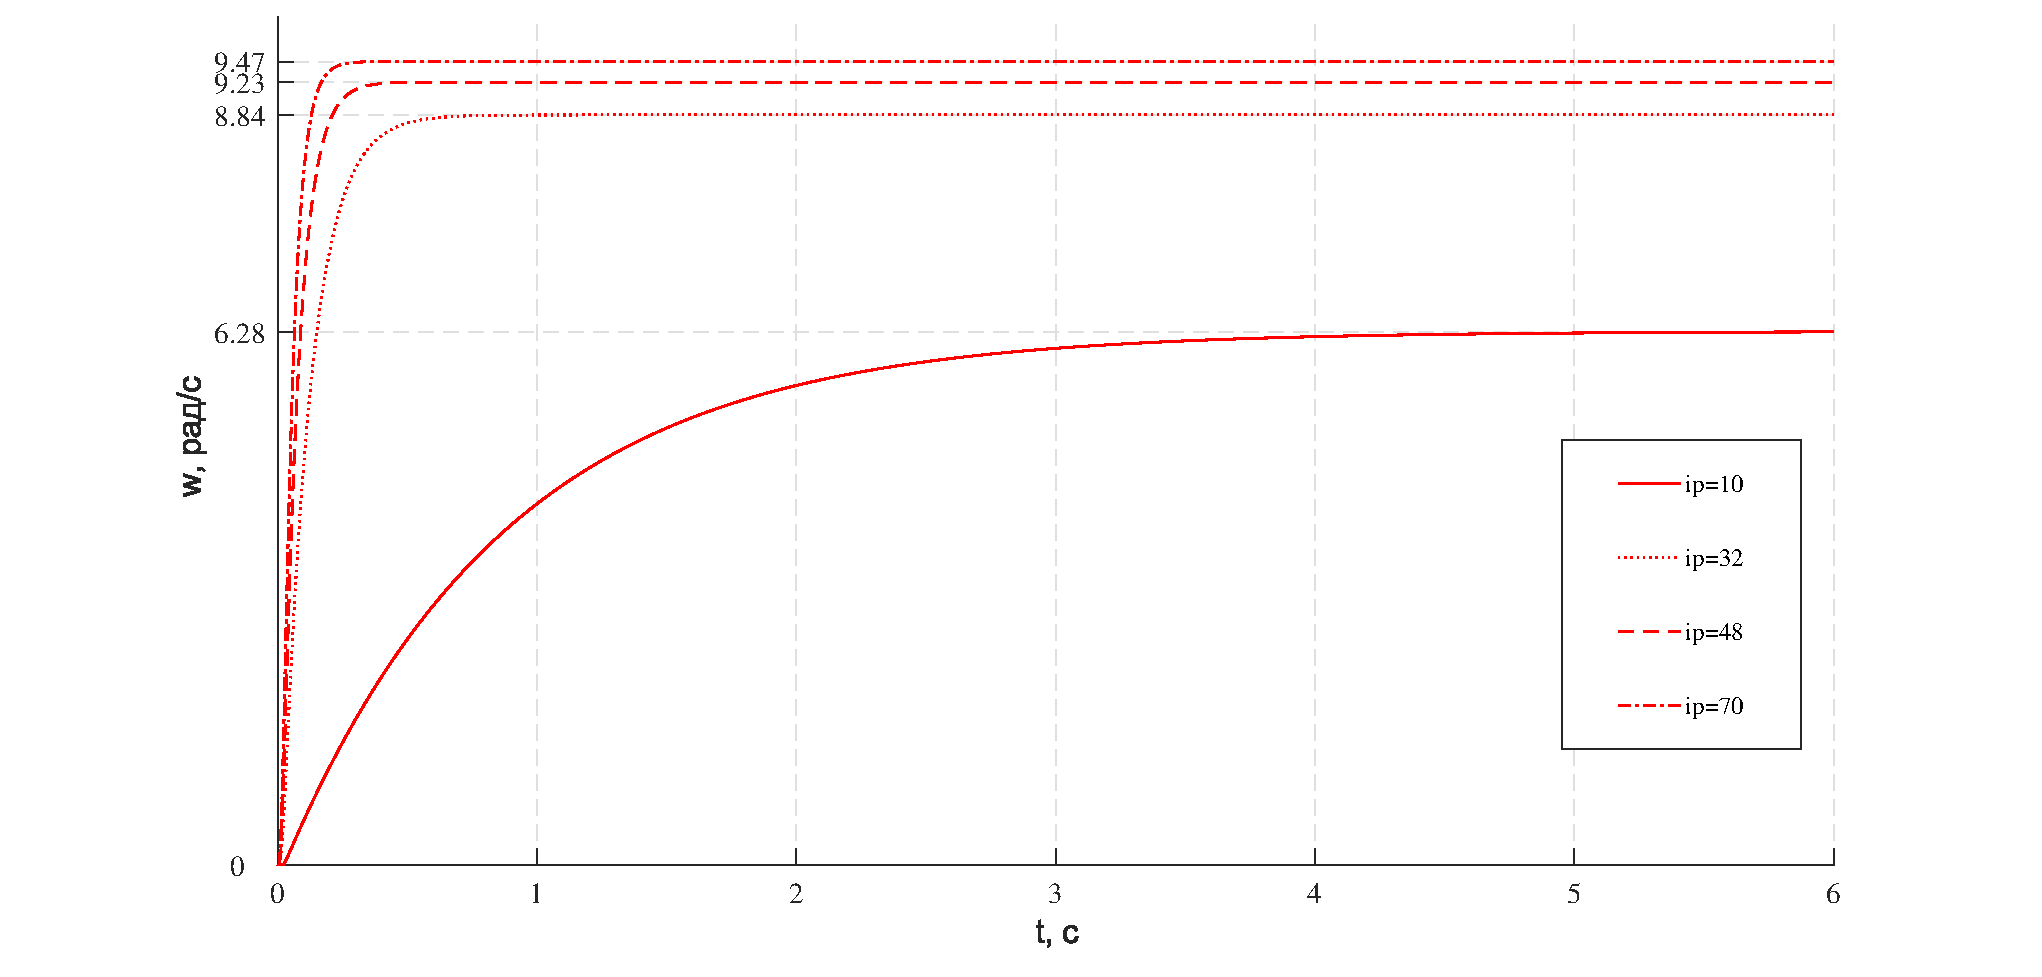
\includegraphics[width=1\linewidth]{new_w_ip_m80.eps}} \\b)
		\end{minipage}
		\vfill
		\begin{minipage}[h]{0.47\linewidth}
			\center{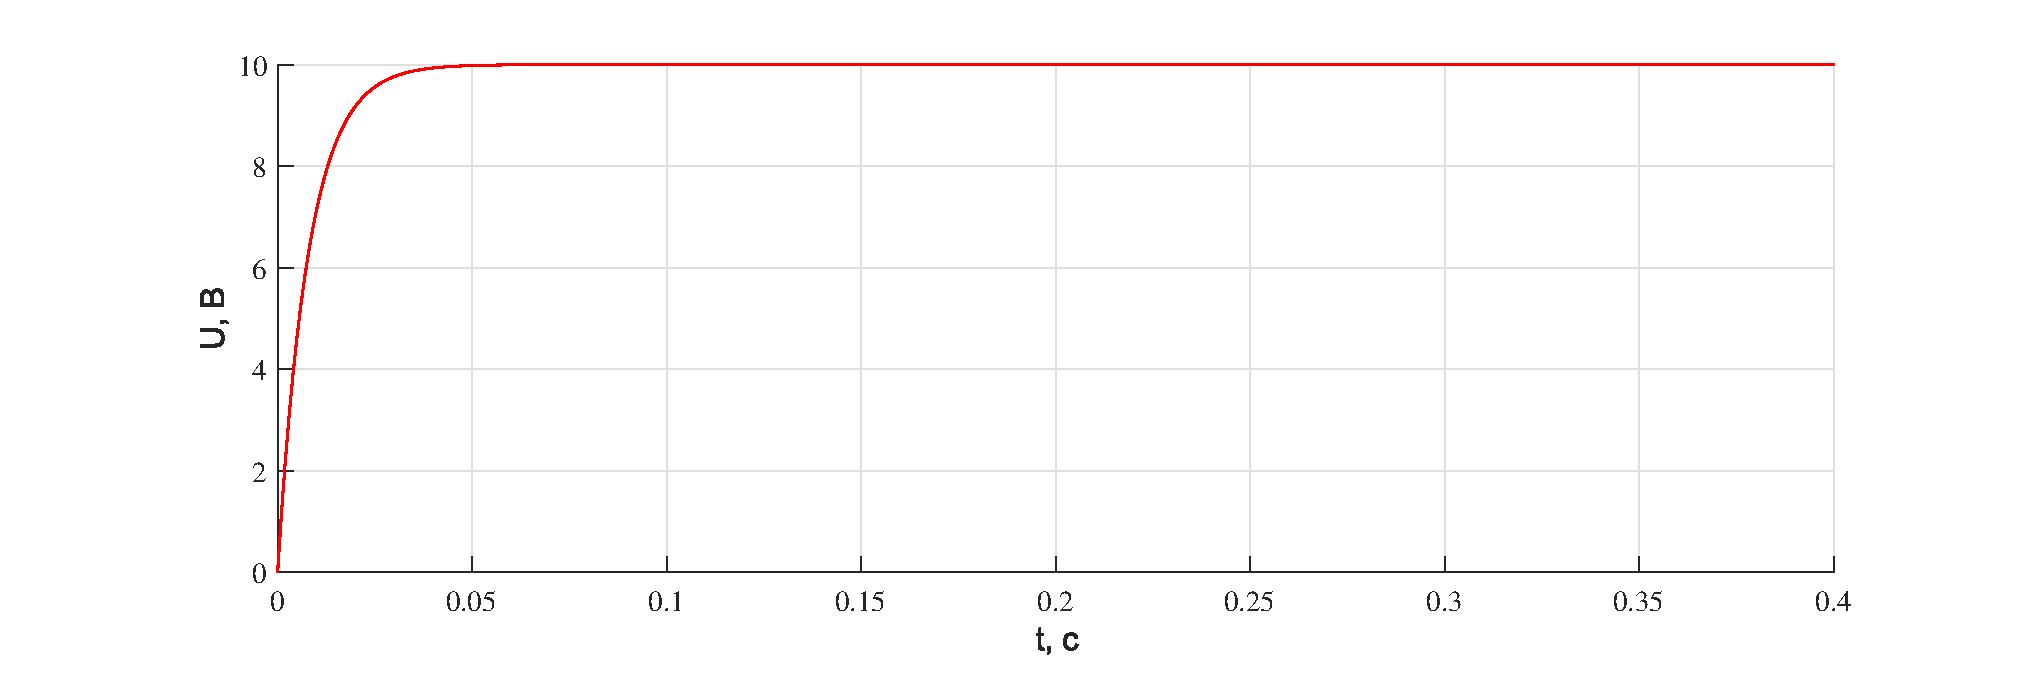
\includegraphics[width=1\linewidth]{new_u_ip_m80.eps}} c) \\
		\end{minipage}
		\hfill
		\begin{minipage}[h]{0.47\linewidth}
			\center{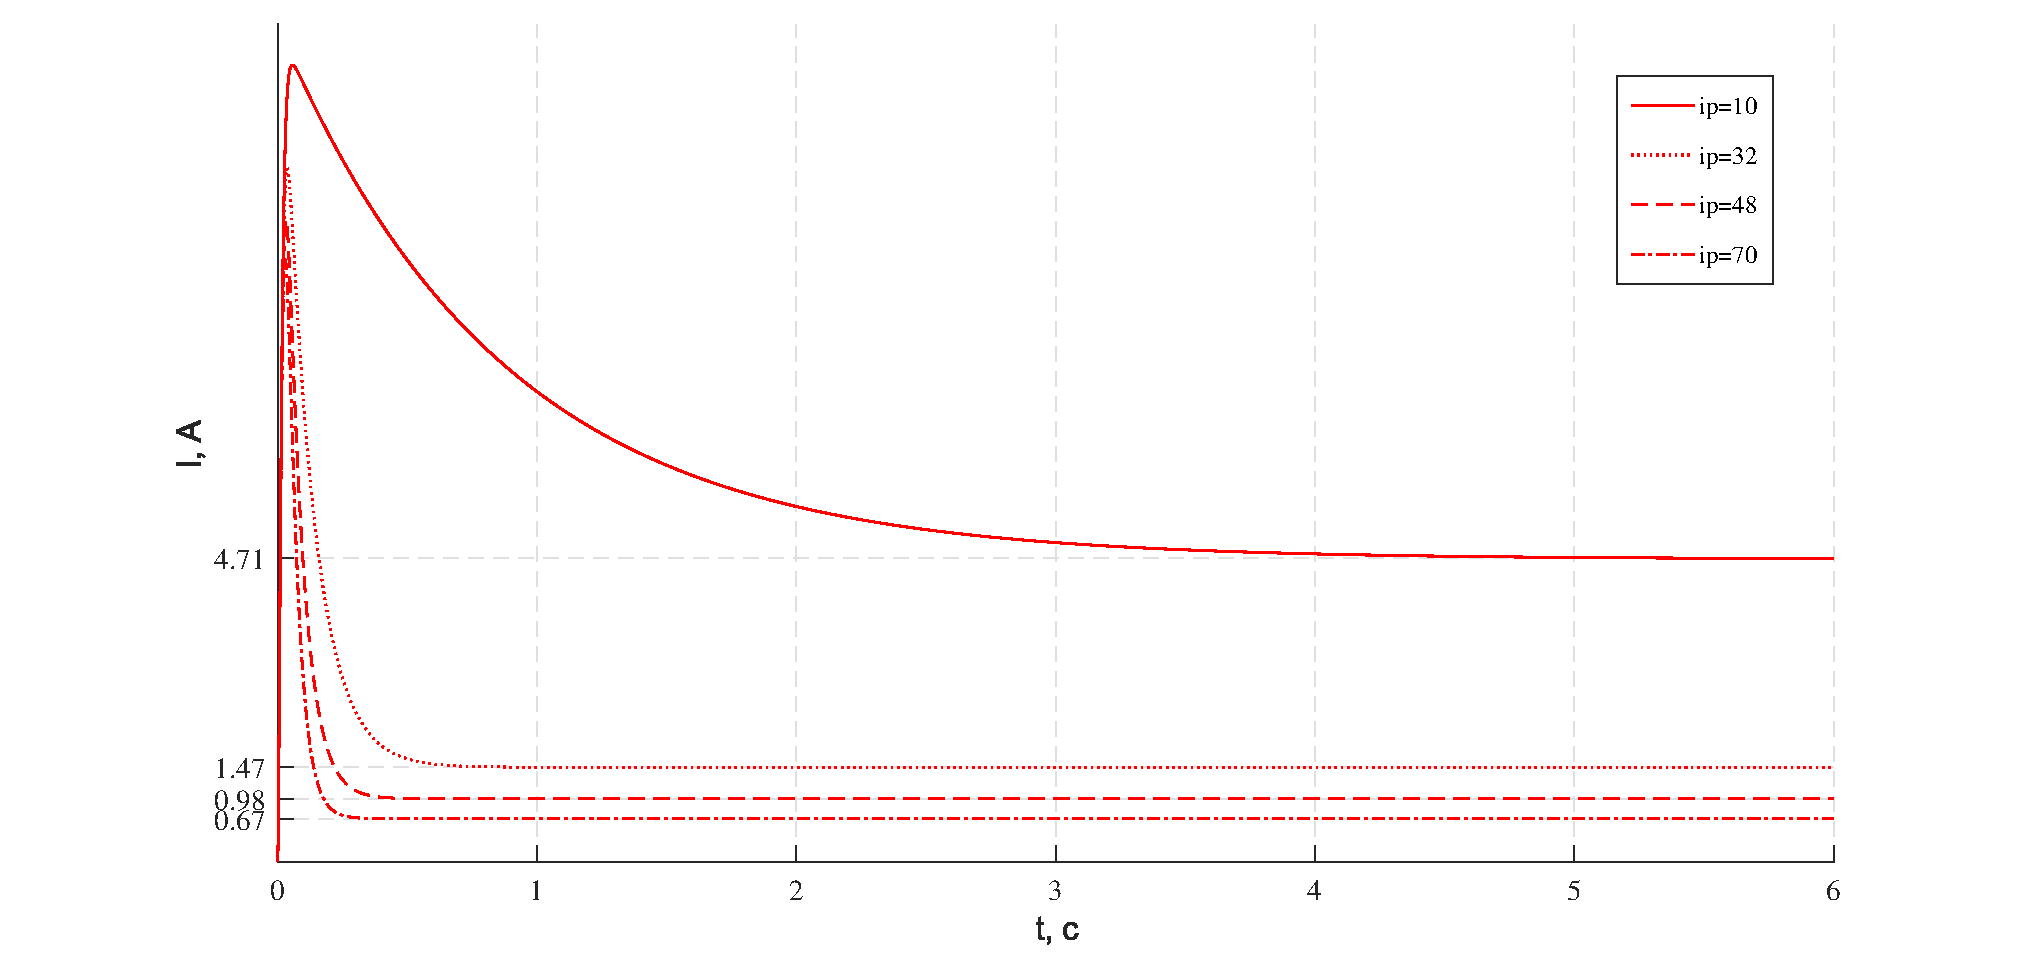
\includegraphics[width=1\linewidth]{new_i_ip_m80.eps}} d) \\
		\end{minipage}
		\caption{Переходные процессы: a) угол поворота, b)
			скорость вращения, c) напряжение, d) сила тока}
		\label{s_6}
	\end{figure}
	\newpage
	\paragraph{}Рассчитаем значения времени переходного процесса $t_\text{п}$ и установившееся значение при различных $i_p$ для $w$ и $I$. Результаты представлены в таблице \ref{t_5}
	\begin{table}[h]
		\caption{Данные моделирования}
		\renewcommand{\arraystretch}{2} 
		\renewcommand{\tabcolsep}{0.5cm}
		\begin{center}
			\begin{tabular}{|c|c|c|c|c|}
				\hline
				\multirow{2}*{$i_p$} & \multicolumn{2}{|c|}{$t_\text{п}$} & \multicolumn{2}{|c|}{Установившееся значение} \\ \cline{2-5}
				& $w$ & $I$ & $w$ & $I$ \\ \hline
				10 & 2.59 & 3 & 6.28 & 4.71\\ \hline
				32 & 0.34 & 0.56 & 8.84 & 1.47\\ \hline
				48 & 0.2 & 0.36 & 9.23 & 0.98\\ \hline
				70 & 0.14 & 0.27 & 9.47 & 0.67\\ \hline
				
			\end{tabular}
		\end{center}
		\label{t_5}
	\end{table}
	\newpage
	\begin{center}
	\section{Исследование упрощенной математической модели ЭМО}
	\end{center}
	\paragraph {} Схема моделирования представлена на рисунке \ref{s_7}
	
	\begin{figure}[h]
		\renewcommand{\figurename}{Рисунок}
		\centering
		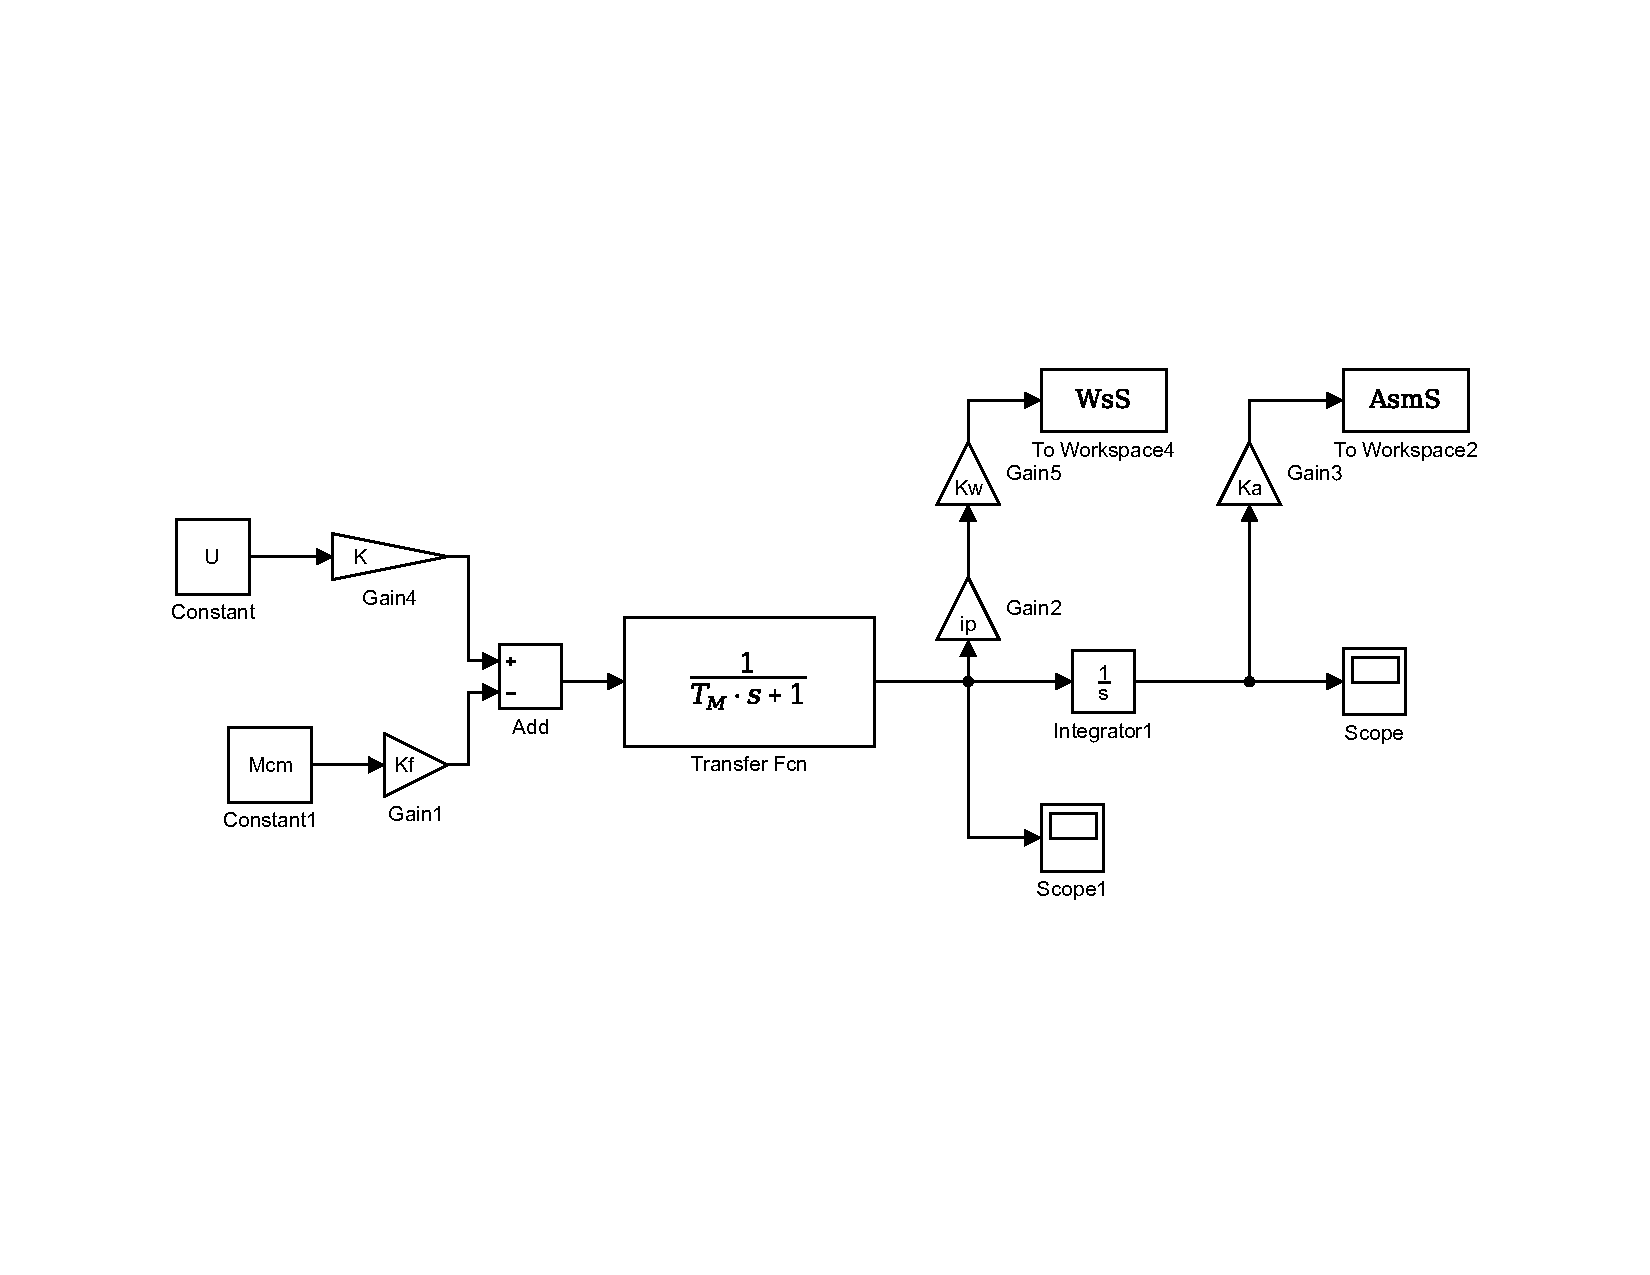
\includegraphics[width=6in]{Lab10Simple2.pdf}
		\caption{Схема моделирования}
		\label{s_7}
	\end{figure}
	\newpage
	Графики переходных процессов для $w$ и $\alpha$ при $U=5$ и $M_{\text{см}}=0$ для упрошенной модели и полной при различных значениях $T_{\text{я}}$ и $T_y$ представлены на рисунках \ref{s_8} и \ref{s_9} соответственно.
	\begin{figure}[h!]
		
		
				\centering
				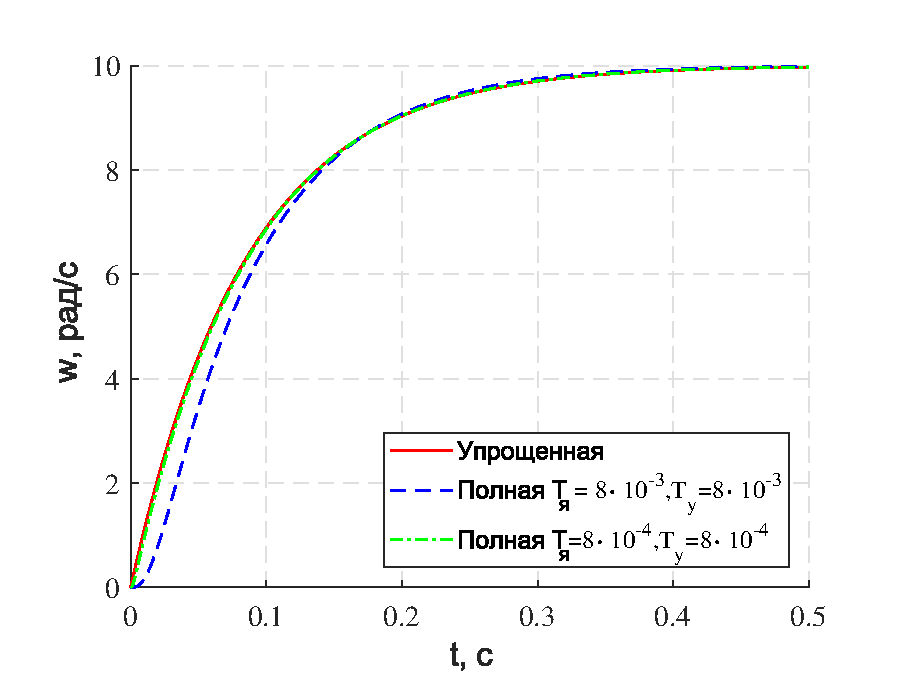
\includegraphics[width=5in]{comparew.eps}
				\caption{Переходные процессы $w$} 
				\label{s_8} 
					\end{figure}
			\begin{figure}[h!]
				\centering
				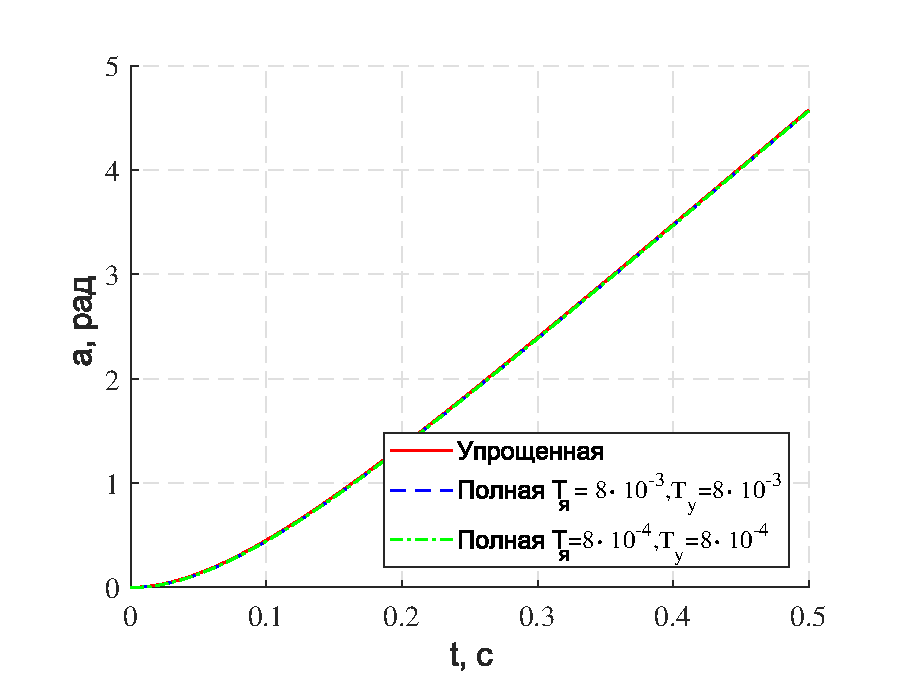
\includegraphics[width=5in]{comparea.eps}
				\caption{Переходные процессы$\alpha$}
				\label{s_9}
			
	\end{figure}
	\newpage
	\begin{center}
	\section{Вывод математических моделей вход-состояние-выход}
	\end{center}
	\paragraph{Полная модель}~\\
	Полная модель данного ЭМО может быть описана следующей системой:\\
	\begin{equation}
	\begin{cases}
	\dot{X}=A\cdot X + B\cdot u 
	\\
	y = C\cdot X + D\cdot u
	\end{cases}
	\end{equation}
	Возьмем в качестве вектора состояния $X=\begin{bmatrix}
	U_y & \\
	I &\\
	w &\\
	\alpha
	\end{bmatrix}$
	~, а за вектор возмущающих воздействий $u=\begin{bmatrix}
	U \\
	M_{\text{см}}\\ \end{bmatrix}$ \\
	
	\noindent Выходная величина $y=\alpha ~\Rightarrow~ C=\begin{bmatrix}
		0 & 0 & 0 & 1\\ \end{bmatrix} ~~D=0$ \\
		Матрицы $A$ и $B$ найдем, используя схему модели. Получаем:\\ 
		\begin{gather}
		\displaystyle A=\begin{bmatrix}
		-\frac{1}{T_y} & 0 & 0 & 0\\
		\frac{K_{\text{д}}}{T_{\text{я}}} & -\frac{1}{T_{\text{я}}} & -\frac{K_e \cdot K_{\text{д}}}{T_{\text{я}}} & 0\\
		0 & \frac{K_M}{J_{\sum}} & 0 & 0\\
		0 & 0 & 1 & 0
		\end{bmatrix} 
		\\ B=\begin{bmatrix}
		-\frac{K_y}{T_y} & 0 \\
		0 & 0 \\
		0 & -\frac{1}{i_p \cdot J_{\sum}} \\
		0 & 0\\
		\end{bmatrix}
		\end{gather}
		
		
		
		\paragraph{Упрощенная модель}~\\
		Упрощенная модель данного ЭМО может быть описана следующей системой:\\
		\begin{equation}
		\begin{cases}
		\dot{X}=A\cdot X + B\cdot u 
		\\
		y = C\cdot X + D\cdot u
		\end{cases}
		\end{equation}
		Возьмем в качестве вектора состояния $X=\begin{bmatrix}
		w &\\
		\alpha
		\end{bmatrix}$
		~, а за вектор возмущающих воздействий $u=\begin{bmatrix}
		U \\
		M_{\text{см}}\\ \end{bmatrix}$ \\
		
		\noindent Выходная величина $y=\alpha ~\Rightarrow~ C=\begin{bmatrix}
		0 & 1\\ \end{bmatrix} ~~D=0$ \\
		Матрицы $A$ и $B$ найдем, используя схему упрощенной модели. Получаем:\\ 
		\begin{gather}
		\displaystyle A=\begin{bmatrix}
		-\frac{1}{T_M} & 0 \\
		1 & 0\\
		\end{bmatrix}\\ B=\begin{bmatrix}
		\frac{K}{T_M} & -\frac{K_f}{T_M} \\
		0 & 0 \\
		\end{bmatrix}
		\end{gather}
	\newpage
	\begin{center}
	\section{Выводы} 
	\end{center}
	\par
	В данной работе была исследована математическая модель электромеханического объекта управления. Были выявлены зависимости переходных процессов от различных параметров. Так, при увеличении момента сопротивления установившееся значение тока якоря увеличивается, а скорости - уменьшается. При увеличении момента инерции механизма время переходного процесса скорости вращения двигателя и среднее значение тока за время своего переходного процесса увеличиваются. При уменьшении передаточного числа редуктора при нулевом моменте сопротивления увеличивается время переходных процессов. А при ненулевом моменте сопротивления увеличивается значение установившегося тока и уменьшается значение скорости. 
	\par
	Также было произведено сравнение упрощенной и полной модели ЭМО. Было показано при моделировании, что если электрические постоянные времени малы по сравнению с механическими, то ими можно пренебречь и перейти от полной к упрощенной модели ЭМО. Также был произведен расчет математических моделей вход-состояние-выход полной и упрощенной модели ЭМО. 





 
\end{document}